\begin{minipage}[b]{0.3\linewidth}
    \centering
    \begin{tikzpicture}[->,>=stealth',node distance=5cm]
      \tikzstyle{every state}=[fill=red!50,draw=none]
      \node[state, scale=0.8] (A)    {$0$};
      \path (A) edge [loop above] node {\footnotesize{(0, 1, $-90^\circ$)}} (A)
                edge [loop below] node {\footnotesize{(0,-1,$-90^\circ$)}} (A);
    \end{tikzpicture}
    \caption{Lattice graph A.}
    \label{fig:lg1}
  \end{minipage}
  \begin{minipage}[b]{0.3\linewidth}
    \centering
    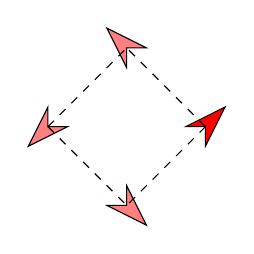
\begin{tikzpicture}
    \draw[fill=red] (3,3) -- (2.75,3) -- (3.25,3.25) -- (3,2.75) -- cycle;
    \draw[fill=red!50] (1,3) -- (1,3.25) -- (0.75,2.75) -- (1.25,3)  -- cycle;
    \draw[fill=red!50] (2.25,1.75) -- (2,2.25) -- (2,2) -- (1.75,2) -- cycle;
    \draw[fill=red!50] (1.75,4.25) -- (2,3.75) -- (2, 4) -- (2.25,4) --  cycle;
    \draw[dashed](1,3) -- (2,4);
    \draw[dashed](3,3) -- (2,4);
    \draw[dashed](3,3) -- (2,2);
    \draw[dashed](1,3) -- (2,2);
  \end{tikzpicture}
  \caption{A square lattice satisfies graph A.}
  \label{fig:lat1}
  \end{minipage}
  \begin{minipage}[b]{0.3\linewidth}
    \centering
    \begin{tikzpicture}[->,>=stealth',node distance=5cm]
      \tikzstyle{every state}=[fill=red!50,draw=none]
      \node[state, scale=0.8] (A)    {$0$};
      \path (A) edge [loop above] node {\footnotesize{(1,0, $45\sqrt{2}^\circ$)}} (A)
                edge [loop below] node {\footnotesize{(-1,0,$-45\sqrt{2}^\circ$)}} (A);
    \end{tikzpicture}
    \caption{Lattice graph B.}
    \label{fig:lg2}
\end{minipage}